\documentclass[tikz,border=12pt]{standalone}
\usepackage[T1]{fontenc}
\usepackage{mathpazo}
\usepackage{amsmath,amssymb}
\usetikzlibrary{arrows.meta, positioning, calc}

\definecolor{stblue}{HTML}{7B97AD}
\definecolor{rwgold}{HTML}{B8995E}
\definecolor{sage}{HTML}{7A9A7E}
\definecolor{dkbrown}{HTML}{3D3530}
\definecolor{wmgray}{HTML}{7B7067}
\definecolor{cream}{HTML}{F9F6F0}
\definecolor{border}{HTML}{D4C9B8}

\begin{document}
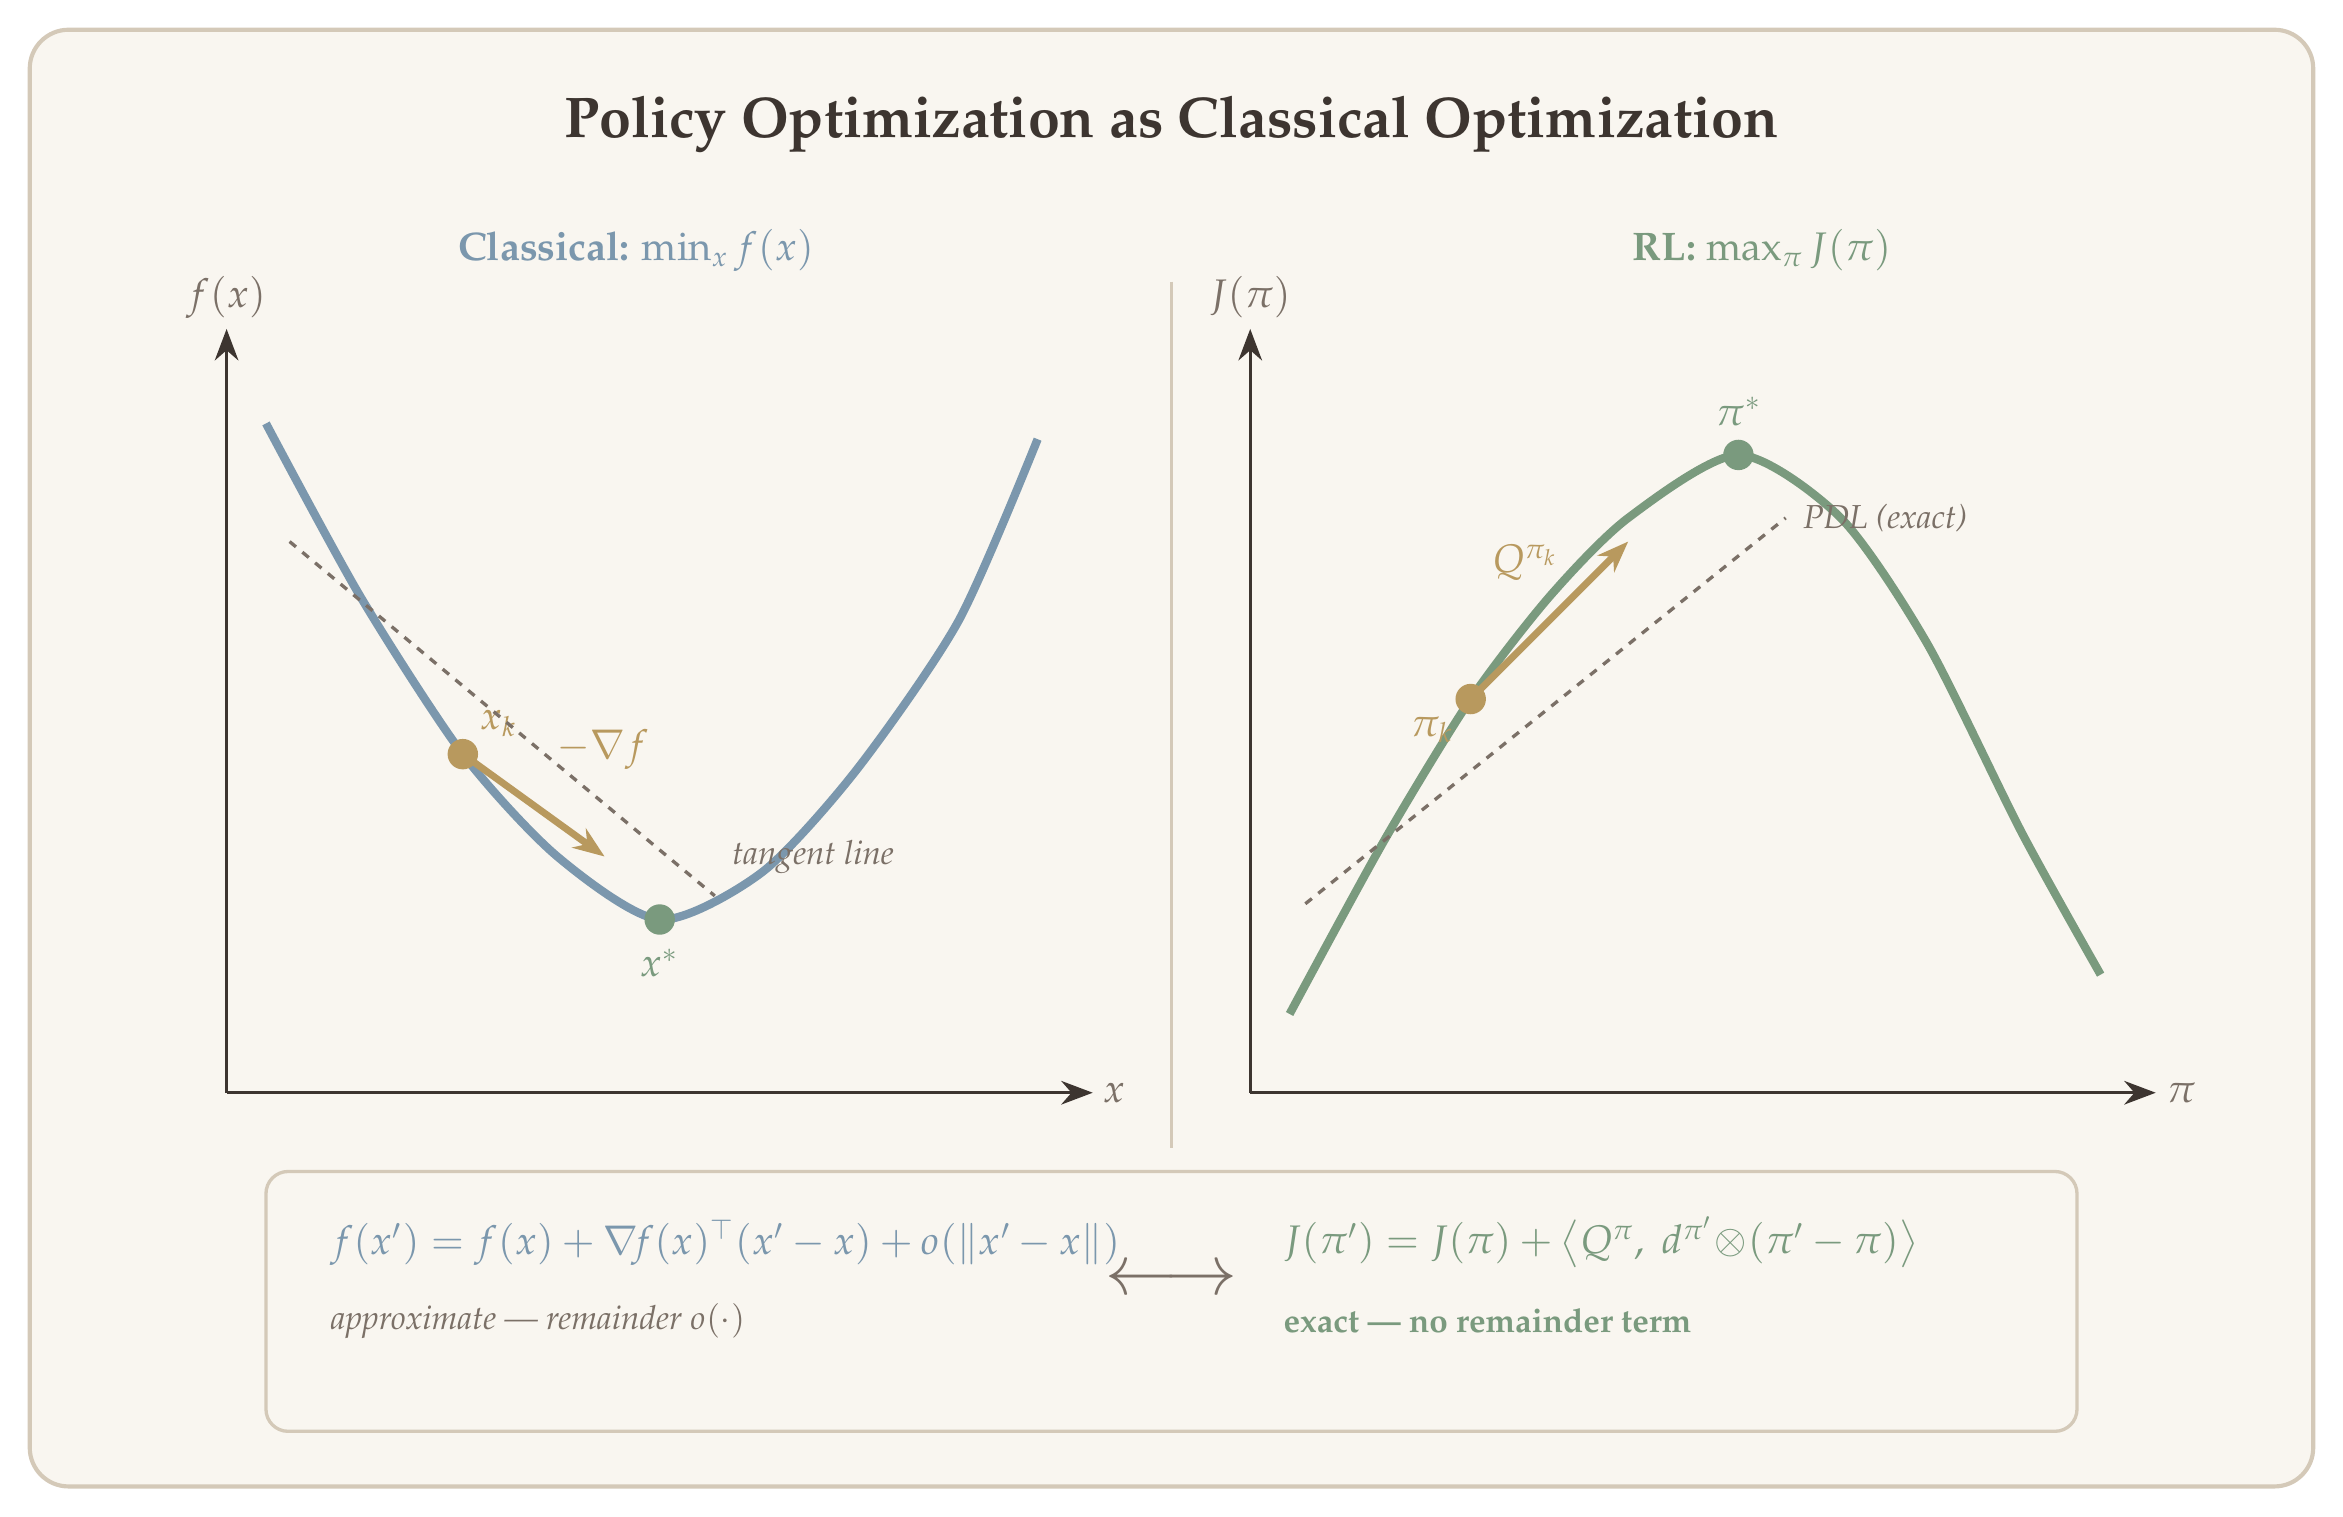
\begin{tikzpicture}[
  >={Stealth[length=4mm, width=3mm]},
]

% Background
\fill[cream, rounded corners=14pt] (-2.5,-8.5) rectangle (26.5,10.0);
\draw[border, rounded corners=14pt, line width=1.5pt] (-2.5,-8.5) rectangle (26.5,10.0);

% Title
\node[font=\huge\bfseries, text=dkbrown] at (12.0,8.8)
  {Policy Optimization as Classical Optimization};

% ========================================
% Left panel: Classical Optimization
% ========================================
\node[font=\Large\bfseries, text=stblue] at (5.2,7.2) {Classical: $\min_x f(x)$};

% Axes
\draw[->, line width=1.2pt, dkbrown] (0,-3.5) -- (11.0,-3.5)
  node[right, font=\Large, text=wmgray] {$x$};
\draw[->, line width=1.2pt, dkbrown] (0,-3.5) -- (0,6.2)
  node[above, font=\Large, text=wmgray] {$f(x)$};

% Convex curve
\draw[stblue, line width=3pt, smooth, tension=0.45]
  plot coordinates {
    (0.5, 5.0)
    (1.7, 2.8)
    (3.0, 0.8)
    (4.2, -0.5)
    (5.5, -1.3)
    (6.8, -0.7)
    (8.0, 0.6)
    (9.3, 2.5)
    (10.3, 4.8)
  };

% Current point x_k
\fill[rwgold] (3.0, 0.8) circle (5.5pt);
\node[font=\Large\bfseries, text=rwgold, above right=4pt] at (3.0,0.8) {$x_k$};

% Optimal point x*
\fill[sage] (5.5, -1.3) circle (5.5pt);
\node[font=\Large\bfseries, text=sage, below=7pt] at (5.5,-1.3) {$x^*$};

% Gradient arrow
\draw[->, rwgold, line width=2.5pt] (3.0, 0.8) -- (4.8, -0.5);
\node[font=\Large\bfseries, text=rwgold, above right=3pt] at (4.0,0.4) {$-\nabla f$};

% Tangent line
\draw[wmgray, line width=1.2pt, dashed] (0.8, 3.5) -- (6.2, -1.0);
\node[font=\large\itshape, text=wmgray, anchor=west] at (6.3,-0.5) {tangent line};

% ========================================
% Right panel: Policy Optimization
% ========================================
\node[font=\Large\bfseries, text=sage] at (19.5,7.2) {RL: $\max_\pi J(\pi)$};

% Axes
\draw[->, line width=1.2pt, dkbrown] (13.0,-3.5) -- (24.5,-3.5)
  node[right, font=\Large, text=wmgray] {$\pi$};
\draw[->, line width=1.2pt, dkbrown] (13.0,-3.5) -- (13.0,6.2)
  node[above, font=\Large, text=wmgray] {$J(\pi)$};

% Performance landscape
\draw[sage, line width=3pt, smooth, tension=0.45]
  plot coordinates {
    (13.5, -2.5)
    (14.7, -0.3)
    (15.8, 1.5)
    (16.8, 2.8)
    (17.8, 3.8)
    (19.2, 4.6)
    (20.5, 3.8)
    (21.6, 2.2)
    (22.8, -0.2)
    (23.8, -2.0)
  };

% Current policy pi_k
\fill[rwgold] (15.8, 1.5) circle (5.5pt);
\node[font=\Large\bfseries, text=rwgold, below left=4pt] at (15.8,1.5) {$\pi_k$};

% Optimal policy pi*
\fill[sage] (19.2, 4.6) circle (5.5pt);
\node[font=\Large\bfseries, text=sage, above=7pt] at (19.2,4.6) {$\pi^*$};

% Q-function arrow
\draw[->, rwgold, line width=2.5pt] (15.8, 1.5) -- (17.8, 3.5);
\node[font=\Large\bfseries, text=rwgold, above left=3pt] at (17.1,2.8) {$Q^{\pi_k}$};

% PDL tangent
\draw[wmgray, line width=1.2pt, dashed] (13.7, -1.1) -- (19.8, 3.8);
\node[font=\large\itshape, text=wmgray, anchor=west] at (19.9,3.8) {PDL (exact)};

% ========================================
% Divider
% ========================================
\draw[border, line width=1.2pt] (12.0,6.8) -- (12.0,-4.2);

% ========================================
% Bottom: Formula comparison
% ========================================
\draw[border, line width=1.2pt, rounded corners=8pt, fill=cream]
  (0.5,-7.8) rectangle (23.5,-4.5);

\node[font=\Large, text=stblue, anchor=west] at (1.2,-5.4)
  {$f(x') = f(x) + \nabla\! f(x)^\top(x' - x) + o(\|x' - x\|)$};
\node[font=\large\itshape, text=wmgray, anchor=west] at (1.2,-6.4)
  {approximate --- remainder $o(\cdot)$};

\node[font=\Huge\bfseries, text=wmgray] at (12.0,-5.9)
  {$\longleftrightarrow$};

\node[font=\Large, text=sage, anchor=west] at (13.3,-5.4)
  {$J(\pi') = J(\pi) + \bigl\langle Q^\pi,\; d^{\pi'} \!\otimes\! (\pi' - \pi)\bigr\rangle$};
\node[font=\large\bfseries, text=sage, anchor=west] at (13.3,-6.4)
  {exact --- no remainder term};

\end{tikzpicture}
\end{document}
